\section{Hashfunktionen}

\begin{frame}
	\frametitle{Was sie tun}
	Eigenschaften
	\begin{columns}
	\column{6cm}
		\begin{itemize}
			\item Surjektiv \begin{small}(Eindeutige Abbildung)\end{small}
			\item Kollisionsfrei
			\item Lawineneffekt
		\end{itemize}
	\column{6cm}
		\begin{center}
			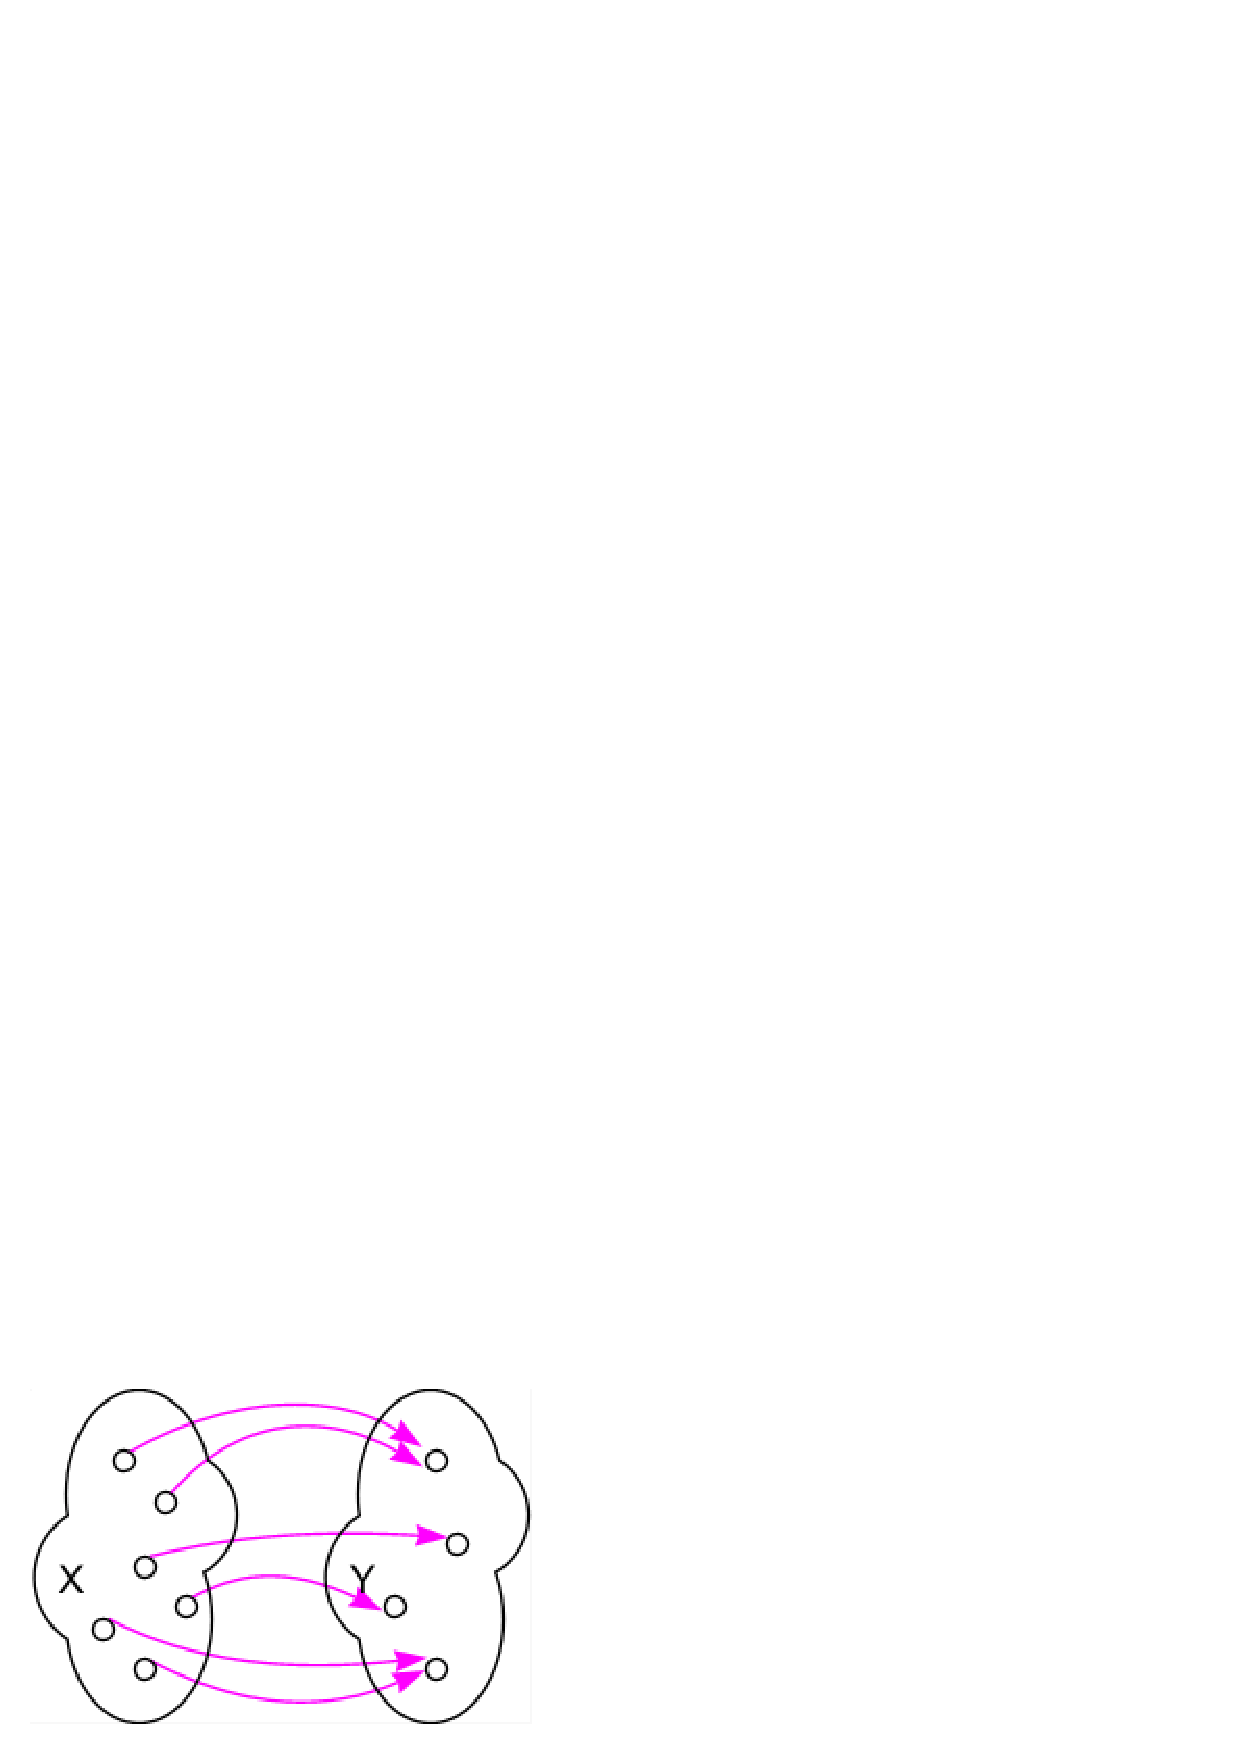
\includegraphics[width=4.8cm,height=3.2cm]{surjektiv}
		\end{center}
	\end{columns}
\end{frame}

\begin{frame}
	\frametitle{Wof"ur?}
	Was bringt's?
	\begin{itemize}
		\item Integrit"at
		\item Authenzit"at \small{(eingeschr"ankt)}
	\end{itemize}

\end{frame}

\begin{frame}
\frametitle{Warum?}
	\begin{columns}
	\column{6cm}
		\begin{itemize}
			\item One-way Eigenschaft
			\item Sinnvoll f"ur gro"se Nachrichten
		\end{itemize}
	\column{6cm}
		\begin{center}
			
\includegraphics[width=4cm,height=6cm]{oneway}
		\end{center}
	\end{columns}
\end{frame}

\begin{frame}
\frametitle{Wie?}
	Signieren mit gemeinsamen Schl"ussel
	\par
	\center{\large{\texttt{hash ( key | nachricht )}}}
\end{frame}

\end{document}
